\documentclass[final]{beamer}

\usepackage[absolute,overlay]{textpos}

\usepackage[utf8]{inputenc}
\usepackage[frenchb]{babel}
\usepackage{verbatim}
\usepackage{graphicx}
\usepackage{color}
\usepackage{hyperref}
\usepackage{verbatim}
\usepackage{url}

\usepackage[pdf]{pstricks}


\usepackage{pifont}
\newcommand{\cmark}{\ding{51}}%
\newcommand{\xmark}{\ding{55}}%

\usepackage{multirow}

\hypersetup{colorlinks=true, linkcolor=black, urlcolor=blue}
\beamertemplatenavigationsymbolsempty
\setbeamertemplate{sections/subsections in toc}[circle]

\selectcolormodel{cmyk}


\setlength{\TPHorizModule}{\paperwidth}
\setlength{\TPVertModule}{\paperheight}

\definecolor{i6blue}{cmyk}{1,0.305,0,0.06}
\definecolor{i6bluedark}{rgb}{0.0156,0.2578,0.5625}
\definecolor{i6colorscheme1}{HTML}{FFFFFF}  % e.g. for block title
\definecolor{i6colorblockbg}{HTML}{ADDFFF}
\definecolor{i6colorblockfg}{HTML}{FFFFFF}
\definecolor{i6colorscheme2}{HTML}{100D09}  % e.g. title in headline
\definecolor{i6colorscheme3}{HTML}{FFFFFF}  % e.g. for poster background
\definecolor{i6colorscheme4}{HTML}{000000}
\definecolor{i6colorschemeHeadline}{HTML}{FFFFFF}  % for headline bg
\definecolor{i6colorschemeFootline}{HTML}{100D09}  % for headline bg

\setbeamercolor{headline}{fg=blue,bg=i6colorschemeHeadline}
\setbeamercolor{title in headline}{fg=blue}
\setbeamercolor{author in headline}{fg=black}
\setbeamercolor{institute in headline}{fg=lightgray}
\setbeamercolor{logo in headline}{fg=black,bg=lightgray}
\setbeamercolor{separation line}{bg=i6colorscheme1}

\definecolor{lightgreen}{rgb}{0.0,0.8,0.0}
\definecolor{lightblue}{rgb}{0.3,0.8,1.0}
\definecolor{lightred}{rgb}{0.874,0.180,0.105}
\definecolor{gray}{rgb}{0.4,0.4,0.4}
\definecolor{lightgray}{rgb}{0.8,0.8,0.8}
\definecolor{shadecolor}{rgb}{0.9,0.9,0.9}


\title{Simple connectome inference from partial correlation statistics\\in calcium imaging}
\author{{\footnotesize Antonio Sutera, Arnaud Joly, Vincent François-Lavet, Zixiao Aaron Qiu, Gilles Louppe, Damien Ernst and Pierre Geurts.}}
\date{}

\addtobeamertemplate{navigation symbols}{}{%
    \usebeamerfont{footline}%
    \usebeamercolor[fg]{footline}%
    \hspace{1em}%
    \insertframenumber/\inserttotalframenumber
}

\begin{document}

%% Slide 1 ==================================================================

\begin{frame}

  \begin{beamercolorbox}[wd=\paperwidth, ignorebg]{headline}
    \begin{center}
      
      \usebeamercolor{title in headline}{\color{fg}\large{\textbf{\inserttitle}}\\[1ex]}
      \usebeamercolor{author in headline}{\color{fg}\footnotesize{\insertauthor}\\[1ex]}
    \end{center}
  \end{beamercolorbox}

\textbf{{\color{i6blue}Goal:}} From time-series of the neuron activity, \textbf{infer} the directed \textbf{connections between neurons}.\\[1ex]
%This is {\color{red} difficult} task.\\[2ex]
\textbf{{\color{i6blue}Results:}} Our method was the \textbf{best} performer in the recent \textit{Neural Connectomics Challenge}.\\[1ex]

\begin{columns}
\begin{column}{0.55\linewidth}
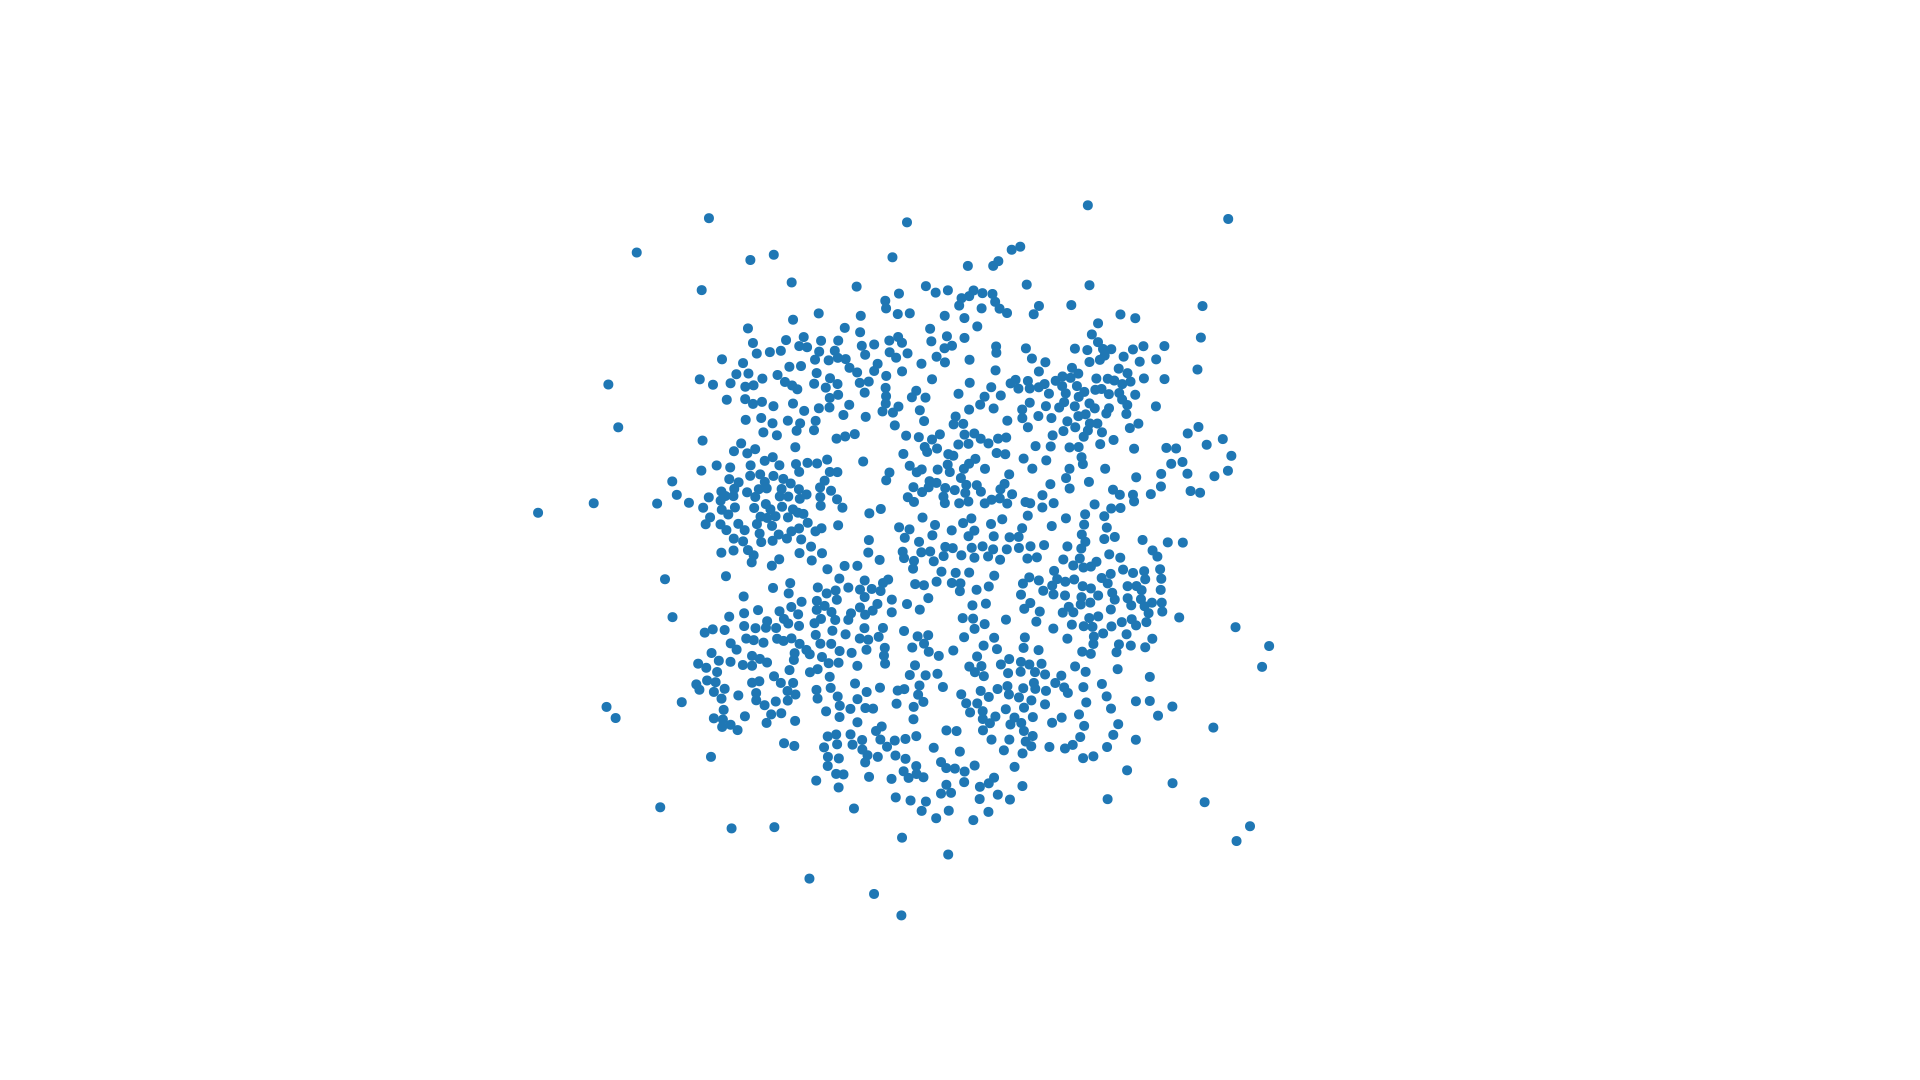
\includegraphics[width=6cm]{images/network.pdf}
\end{column}
\begin{column}{0.5\linewidth}

\textbf{{\color{green} Steps of our solution:}}
\begin{enumerate}[{\color{i6blue} 1.}]
\item Signal processing\\{\scriptsize(deal with calcium fluorescent signals)}
\item Averaged partial correlation statistics\\{\scriptsize(find the undirected network)}
\item Prediction of edge orientation
\end{enumerate}


\end{column}
\end{columns}


\end{frame}

\end{document}